% Options for packages loaded elsewhere
\PassOptionsToPackage{unicode}{hyperref}
\PassOptionsToPackage{hyphens}{url}
\PassOptionsToPackage{dvipsnames,svgnames,x11names}{xcolor}
\documentclass[
  11pt,
]{article}
\usepackage{xcolor}
\usepackage[margin=1in]{geometry}
\usepackage{amsmath,amssymb}
\setcounter{secnumdepth}{5}
\usepackage{iftex}
\ifPDFTeX
  \usepackage[T1]{fontenc}
  \usepackage[utf8]{inputenc}
  \usepackage{textcomp} % provide euro and other symbols
\else % if luatex or xetex
  \usepackage{unicode-math} % this also loads fontspec
  \defaultfontfeatures{Scale=MatchLowercase}
  \defaultfontfeatures[\rmfamily]{Ligatures=TeX,Scale=1}
\fi
\usepackage{lmodern}
\ifPDFTeX\else
  % xetex/luatex font selection
\fi
% Use upquote if available, for straight quotes in verbatim environments
\IfFileExists{upquote.sty}{\usepackage{upquote}}{}
\IfFileExists{microtype.sty}{% use microtype if available
  \usepackage[]{microtype}
  \UseMicrotypeSet[protrusion]{basicmath} % disable protrusion for tt fonts
}{}
\usepackage{longtable,booktabs,array}
\usepackage{caption}
\captionsetup[table]{skip=6pt}
\newcounter{none} % for unnumbered tables
\usepackage{calc} % for calculating minipage widths
% Correct order of tables after \paragraph or \subparagraph
\usepackage{etoolbox}
\makeatletter
\patchcmd\longtable{\par}{\if@noskipsec\mbox{}\fi\par}{}{}
\makeatother
\usepackage{graphicx}
\makeatletter
\newsavebox\pandoc@box
\newcommand*\pandocbounded[1]{% scales image to fit in text height/width
  \sbox\pandoc@box{#1}%
  \Gscale@div\@tempa{\textheight}{\dimexpr\ht\pandoc@box+\dp\pandoc@box\relax}%
  \Gscale@div\@tempb{\linewidth}{\wd\pandoc@box}%
  \ifdim\@tempb\p@<\@tempa\p@\let\@tempa\@tempb\fi% select the smaller of both
  \ifdim\@tempa\p@<\p@\scalebox{\@tempa}{\usebox\pandoc@box}%
  \else\usebox{\pandoc@box}%
  \fi%
}
% Set default figure placement to htbp
\def\fps@figure{htbp}
\makeatother
% definitions for citeproc citations
\NewDocumentCommand\citeproctext{}{}
\NewDocumentCommand\citeproc{mm}{%
  \begingroup\def\citeproctext{#2}\cite{#1}\endgroup}
\makeatletter
 % allow citations to break across lines
 \let\@cite@ofmt\@firstofone
 % avoid brackets around text for \cite:
 \def\@biblabel#1{}
 \def\@cite#1#2{{#1\if@tempswa , #2\fi}}
\makeatother
\newlength{\cslhangindent}
\setlength{\cslhangindent}{1.5em}
\newlength{\csllabelwidth}
\setlength{\csllabelwidth}{3em}
\newenvironment{CSLReferences}[2] % #1 hanging-indent, #2 entry-spacing
 {\begin{list}{}{%
  \setlength{\itemindent}{0pt}
  \setlength{\leftmargin}{0pt}
  \setlength{\parsep}{0pt}
  % turn on hanging indent if param 1 is 1
  \ifodd #1
   \setlength{\leftmargin}{\cslhangindent}
   \setlength{\itemindent}{-1\cslhangindent}
  \fi
  % set entry spacing
  \setlength{\itemsep}{#2\baselineskip}}}
 {\end{list}}
\usepackage{calc}
\newcommand{\CSLBlock}[1]{\hfill\break\parbox[t]{\linewidth}{\strut\ignorespaces#1\strut}}
\newcommand{\CSLLeftMargin}[1]{\parbox[t]{\csllabelwidth}{\strut#1\strut}}
\newcommand{\CSLRightInline}[1]{\parbox[t]{\linewidth - \csllabelwidth}{\strut#1\strut}}
\newcommand{\CSLIndent}[1]{\hspace{\cslhangindent}#1}
\setlength{\emergencystretch}{3em} % prevent overfull lines
\providecommand{\tightlist}{%
  \setlength{\itemsep}{0pt}\setlength{\parskip}{0pt}}
\usepackage{etoolbox}
\AtBeginEnvironment{longtable}{\small\setlength{\tabcolsep}{4pt}}
\usepackage{needspace}
\ifPDFTeX\DeclareUnicodeCharacter{2212}{\textminus}\fi
\usepackage{float}
\floatplacement{figure}{htbp}
\usepackage{bookmark}
\IfFileExists{xurl.sty}{\usepackage{xurl}}{} % add URL line breaks if available
\urlstyle{same}
% fallback for those not using the hyperref driver hyperxmp:
\makeatletter
\@ifundefined{xmpquote}{\newcommand{\xmpquote}[1]{#1}}{}
\makeatother
\hypersetup{
  pdftitle={How Much of the Decline in English Sentence Length Is Punctuation? Evidence from Dated Project Gutenberg Books, 1600--1974},
  pdfauthor={Joe Karlsson},
  pdfkeywords={\xmpquote{sentence length}, \xmpquote{punctuation}, \xmpquote{semicolon}, \xmpquote{historical linguistics}, \xmpquote{Project Gutenberg}, \xmpquote{cultural analytics}},
  colorlinks=true,
  linkcolor={black},
  filecolor={Maroon},
  citecolor={black},
  urlcolor={blue},
  pdfcreator={LaTeX via pandoc}}

\title{How Much of the Decline in English Sentence Length Is Punctuation? Evidence from Dated Project Gutenberg Books, 1600--1974}
\author{Joe Karlsson \\ \small Independent researcher}
\date{November 22, 2026}

\begin{document}
\maketitle
\begin{abstract}
English sentences are said to have shortened by half since the Elizabethans, and linguists have long suspected that part of the decline is a change in punctuation: writers who once joined clauses with
semicolons and colons began ending them with periods. This paper measures how large that part is. In Project Gutenberg books with a known first-publication date, after removing duplicate works, the
median number of words between sentence-final marks (. ? !) falls from 31.1 in 1700--1749 to 14.5 in 1900--1949. A sample of 100 eighteenth-century semicolons and colons was coded for whether each
joins two clauses that could stand as sentences; on the 82 marks from English originals, 72\% of semicolons and 59\% of colons do. Counting each mark as a stop at that rate, the median falls from 23.6
to 13.6 words, so 40\% of the decline disappears (95\% interval 24--51\%, resampling both books and coded marks). Restricted to the 13 books of 1700--1749 whose title pages show them to be English
originals, the share is 45\% (29--53\%). Other weighted variants (dropping plays and poetry, starting at 1750, separate glue rates for each era, and, on the books that still have full texts, stripping
editorial apparatus, a stricter sentence splitter or narration only) give 35--49\%. Removing quoted speech shrinks the remaining decline by about a tenth. The semicolon falls from a median of 10.1 to
1.8 per 1,000 words between 1775--1799 and 1950--1974; publication year and author birth year fit that fall equally well and cannot be separated here. The coding was done by a large language model and
checked by a second, blind model run; a human coder is the main outstanding check. Code, per-book data and coded samples are public.

\textbf{Keywords:} sentence length; punctuation; semicolon; historical linguistics; Project Gutenberg; cultural analytics
\end{abstract}

\section{Introduction}\label{introduction}

In 1894 Edwin Lewis concluded that ``the English sentence has decreased in average length at least one-half in three hundred years'' (\citeproc{ref-Lewis1894}{Lewis 1894}). A year earlier Lucius
Sherman had tallied 41.4 words per sentence in Richard Hooker against 22.5 in Macaulay (\citeproc{ref-Sherman1893}{Sherman 1893}).

The standard objection is about units. A sentence, as most of these studies count it, runs from one period, question mark or exclamation mark to the next. Eighteenth-century writers often joined
independent clauses with semicolons and colons where later writers would put a period. If they did, part of the decline is the same prose cut into more pieces. The objection is widely repeated
(\citeproc{ref-Fahnestock2011}{Fahnestock 2011}; \citeproc{ref-Biber2009}{Biber and Conrad 2009}; both as reviewed in \citeproc{ref-Rudnicka2018}{Rudnicka 2018}; \citeproc{ref-Liberman2022}{Liberman
2022}; \citeproc{ref-Oliver2025}{Oliver 2025}), but I have found no study that measures how much of the decline it explains across the eighteenth and nineteenth centuries, when the semicolon was
common. The one direct test I know of, Westin's comparison of the two ways of counting in twentieth-century British newspaper editorials (\citeproc{ref-Westin2002}{Westin 2002}; as summarized in
\citeproc{ref-Rudnicka2018}{Rudnicka 2018}), found almost no difference, which is consistent with the punctuation explanation if the semicolon had already become rare by then, as Bruthiaux
(\citeproc{ref-Bruthiaux1995}{1995}) suggests it may have.

This paper makes that measurement. It compares two units on the same books: words between sentence-final marks, and words between stops, where semicolons and colons also end a unit. If punctuation
explains part of the decline, the two series should be far apart before 1800 and converge as the semicolon disappears. The share of the decline that vanishes under the second unit is the punctuation
share. A semicolon can also separate list items or subordinate clauses, and a colon can introduce a quotation, so a coded sample gives the rate at which each mark joins clauses that could stand alone
(its \emph{glue rate}), and the estimate counts each mark at that rate.

The corpus is Punc, an art project that strips the words from books and keeps the punctuation, which holds 1,959 Project Gutenberg books. Section 3 describes what that origin means for the corpus.

In brief:

\begin{enumerate}
\def\labelenumi{\arabic{enumi}.}
\tightlist
\item
  About 40\% of the decline from 1700--1749 to 1900--1949 is punctuation (95\% interval 24--51\%; 35--49\% across the other weighted variants; 45\% on 1700--1749 books verified as English originals).
\item
  The rest is not dialogue. With quoted speech removed, the weighted share on narration alone is 45\%, against 42\% for the full texts of the same books.
\item
  The semicolon falls from 10.1 to 1.8 per 1,000 words between 1775--1799 and 1950--1974, steepest after 1825. Publication year and author birth year fit this equally well.
\end{enumerate}

All analyses were chosen after the data were available; none was pre-registered. Section 4 lists the choices made after the first results were seen, including the corrections made after review.

\section{Background}\label{background}

\textbf{Punctuation's history.} Punctuation moved from marking pauses for reading aloud toward marking grammatical structure (\citeproc{ref-Parkes1992}{Parkes 1992}). In a grammatical account, the
semicolon and colon separate units at the level of the clause (\citeproc{ref-Nunberg1990}{Nunberg 1990}). Bruthiaux (\citeproc{ref-Bruthiaux1995}{1995}) traces four centuries of semicolon use in one
genre and argues that ``after flourishing in the seventeenth and eighteenth centuries, the semicolon may have become a marginal component of the English punctuation system.'' Watson
(\citeproc{ref-Watson2019}{2019}) gives the mark's cultural history.

\textbf{Sentence length over time.} Rudnicka (\citeproc{ref-Rudnicka2018}{2018}) tests the assumption of a steady decline in the Corpus of Historical American English and links changes in sentence
length to syntactic change. In the full text it reviews the punctuation objection and reports ``a dramatic decrease in the frequency of use of semicolons happening between 1810 and 1900.'' Liberman
(\citeproc{ref-Liberman2022}{2022}) asks whether the perceived trend would be better titled ``Historical trends in English punctuation practices.'' Register studies complicate the picture: Biber and
Finegan (\citeproc{ref-Biber1989}{1989}) traces fiction, essays and letters along dimensions running between `oral' and `literate' styles over four centuries, and Biber and Gray
(\citeproc{ref-Biber2015}{2015}) shows that grammatical complexity in academic writing moved from embedded clauses into phrases, so a shorter sentence need not be a simpler one. Linguists' alternative
unit, the T-unit, is a main clause plus whatever is attached to it (\citeproc{ref-Hunt1965}{Hunt 1965}); words between stops is a crude version of it.

\textbf{Punctuation as data.} In narrative texts, punctuation marks follow the same statistical laws as words (\citeproc{ref-Kulig2016}{Kulig et al. 2017}), and the spacing between marks follows
regular distributions whose parameters differ by language (\citeproc{ref-Stanisz2023}{Stanisz et al. 2023}). Darmon et al. (\citeproc{ref-Darmon2020}{2020}) uses punctuation sequences from Project
Gutenberg for authorship and genre analysis. None of this work connects the change in punctuation to the sentence-length trend.

\textbf{Generations.} Underwood et al. (\citeproc{ref-Underwood2022}{2022}) finds, in 10,830 works of fiction from 1880 to 1999, that ``slightly more than half (54.7 percent) of the variance explained
by time is explained better by an author's year of birth than by a book's year of publication,'' the cohort-succession mechanism described by Ryder (\citeproc{ref-Ryder1965}{1965}). Whether the
semicolon's decline follows writers' generations has not been tested.

\textbf{Dialogue.} Muzny et al. (\citeproc{ref-Muzny2017}{2017}) models the dialogic character of narration and quotation in 1,100 novels, and in its full text reports more quotation over time. Since
speech is short, more dialogue alone would shorten the average sentence; Section 5.3 removes it.

\section{Data}\label{data}

\textbf{Corpus.} Punc's shelf holds Project Gutenberg's 2,000 most-downloaded English books in the 2026-11-10 snapshot (downloads over the previous 30 days), minus dictionaries, encyclopedias, books
with no plain text and some repeat editions, plus three books listed by hand, all of which were in the top 2,000 anyway (\texttt{paper/hand-added.md}): 1,959 books. Gutenberg's license header and
footer are removed at the \texttt{***\ START} and \texttt{***\ END} lines; editorial matter inside the text (modern prefaces, editors' footnotes and glossaries) is kept in the main analysis and
removed by rule as a check (Section 5.2). Gerlach and Font-Clos (\citeproc{ref-Gerlach2020}{2020}) warns that studies built on hand-picked Gutenberg subsets risk bias and are hard to reproduce; the
live shelf is a rolling ranking that drifts (55 of the 938 books analyzed here have since left it), so the corpus is defined by the frozen book list published with the data, not by the live shelf.

\textbf{Duplicate works.} Among the dated books, 16 were duplicates of 13 works: a second edition of the same work (\emph{Gulliver's Travels}, \emph{The Wealth of Nations}, Franklin's
\emph{Autobiography}, \emph{On the Origin of Species}, \emph{The Adventures of Sherlock Holmes}, Emerson's \emph{Essays}, \emph{The Practice of the Presence of God}) or a further volume of one work
(\emph{Don Quixote}, David Henry's 1774 \emph{Historical Account of All the Voyages Round the World}, \emph{The Magic Ring} and others). Each work is kept once, as its most-downloaded copy
(\texttt{paper/reanalysis.py}). This leaves 938 books dated 1600--1974, removing 1 book from 1700--1749 and 4 from 1750--1799. Table 1 shows the corpus before deduplication; Table 2 and every share in
Section 5.1 and 5.2 use the deduplicated corpus. The rule matches only books with the same author and year, so volumes published in different years (such as \emph{Don Quixote} Part II, 1615) are kept.

\textbf{Dates.} Each book's first-publication year comes from Wikidata (\citeproc{ref-Vrandecic2014}{Vrandečić and Krötzsch 2014}), with a hand-checked override list. Translations take the original's
year, which matters here because a translation's punctuation is the translator's (Section 7). 1,073 of the 1,959 books have a year: 114 before 1600 (excluded from all analyses over time), 954 between
1600 and 1974, and 5 after 1974. Only 67 dated books appeared after 1930, because Gutenberg carries works in the US public domain, which mostly means works published before 1931
(\citeproc{ref-Domain2026}{Duke Center for the Study of the Public Domain 2026}). The trend therefore ends in the mid-twentieth century.

\textbf{Composition.} Table 1 describes the dated books by period. The early periods are small (13 to 48 books before 1800), translations are common before 1850, and plays make up 43\% of 1600--1649.

\needspace{16\baselineskip}

\begin{longtable}[]{@{}lrrrrrrr@{}}
\caption{Dated books by 50-year period, before deduplication. Translated: flagged by Gutenberg's catalog or by the word ``translated'' on the title page. This flag errs both ways: it misses Voltaire's
\emph{Candide} and Rousseau's \emph{Discourse} and \emph{Confessions}, and flags English originals such as Walpole's \emph{Castle of Otranto}. Plays, poetry and novels: Punc's genre tags (a book can
have several or none).}\tabularnewline
\toprule\noalign{}
Period & Books & Translated & Plays & Poetry & Novels & Median words & Median download rank \\
\midrule\noalign{}
\endfirsthead
\toprule\noalign{}
Period & Books & Translated & Plays & Poetry & Novels & Median words & Median download rank \\
\midrule\noalign{}
\endhead
\bottomrule\noalign{}
\endlastfoot
1600--1649 & 21 & 29\% & 43\% & 5\% & 19\% & 23,619 & 618 \\
1650--1699 & 13 & 31\% & 0\% & 8\% & 8\% & 58,695 & 317 \\
1700--1749 & 18 & 28\% & 0\% & 6\% & 56\% & 103,398 & 578 \\
1750--1799 & 48 & 31\% & 2\% & 10\% & 29\% & 71,590 & 462 \\
1800--1849 & 96 & 24\% & 1\% & 8\% & 44\% & 127,067 & 522 \\
1850--1899 & 288 & 22\% & 3\% & 3\% & 41\% & 85,542 & 558 \\
1900--1949 & 445 & 11\% & 2\% & 2\% & 43\% & 68,343 & 645 \\
1950--1974 & 25 & 4\% & 0\% & 0\% & 32\% & 48,511 & 621 \\
\end{longtable}

\textbf{Translation status, 1700--1799.} Because the flag is unreliable, the title page of each of the 61 deduplicated books dated 1700--1799 was read (\texttt{paper/translation-status.csv}; two books
no longer on disk were judged from the catalog). 19 are translations: six by Kant, five by Rousseau, two by Goethe, and one each by Leibniz, Prévost, Holberg, Voltaire and Jean Paul, plus Fielding's
version of Ovid. The other 42 are English originals. The catalog flag disagreed with the title page for 11 of the 61. Books from 1800 on were not checked this way. Some of the 19 are
eighteenth-century English versions (the 1742 English Holberg, Fielding's 1747 Ovid) whose punctuation belongs to the period, so removing all translations removes some period punctuation along with
the anachronistic kind.

\textbf{Selection.} The shelf reflects what readers download now, not what was printed then. If readers today prefer eighteenth-century books that read like modern ones, the early periods would
understate their sentence length. Within 1700--1799 (61 deduplicated books), the Spearman correlation between download rank and words between periods is −0.26, and with weighted words between stops
−0.25: the more-downloaded books (lower rank numbers) have longer sentences. Within 1900--1949 both are −0.05 or −0.06. Rank and the semicolon rate are uncorrelated in both (+0.04). So the shelf does
not make the eighteenth century look more modern. If the same pattern holds below the top 2,000, it may overstate eighteenth-century sentence length instead; because P and the weighted S move
together, the effect on the share is likely smaller than on either series, but with 61 books this is not settled.

\section{Methods}\label{methods}

\textbf{Counting.} Curly quotes and long dashes are folded into their plain forms. Punc ends a sentence at any run of \texttt{.}, \texttt{?} or \texttt{!}. Rates are per 1,000 words. Dialogue is the
share of words inside double quotation marks. A stricter splitter, used as a check, does not end sentences at abbreviations such as ``Mr.'', initials, ellipses or dialogue tags
(\texttt{"Help!"\ he\ cried}). A second narration count also removes text in single quotation marks. Another check removes editorial apparatus by rule: bracketed editorial notes and footnote markers,
footnote paragraphs, transcribers' and producers' notes, introductions, prefaces and memoirs headed or credited as an editor's or translator's, and notes, indexes and glossaries at the end of a book
(\texttt{paper/fulltext\_checks.py}).

\textbf{Two units.} For each book, \emph{words between periods} (P) is words divided by sentence-final marks, and \emph{words between stops} (S) is words divided by sentence-final marks plus
semicolons and colons.

\textbf{The punctuation share.} For a start period \emph{a} and end period \emph{z}, with medians of per-book values, the punctuation share is \(1 - (S_a - S_z)/(P_a - P_z)\): the fraction of the
decline in P that does not appear in S. The main comparison is 1700--1749 to 1900--1949. Table 2's P series peaks in 1700--1749, but that peak is partly an artifact of genre: 9 of the 21 books from
1600--1649 (before deduplication) are plays, which have a median of 8.5 words a sentence across the shelf, and the 10 deduplicated prose books from 1600--1649 have a median P of 37.6, above
1700--1749's prose median of 32.4. Ten books are too few to measure from, so the comparison starts at 1700, and Section 5.2 reports a start at 1750.

\textbf{Glue rates.} 100 marks (60 semicolons, 40 colons) were drawn at random (seed 42) from prose books dated 1700--1799 that Gutenberg's catalog does not list as translations. That check missed
some translations: 18 of the 100 marks come from Rousseau, Voltaire, Kant, Holberg, and Fielding's version of Ovid. The glue rates used here come from the other 82 marks (50 semicolons, 32 colons).
Each mark was coded for one question: could the text after the mark stand as its own sentence? The first coder's rule allowed \emph{and}, \emph{but} and \emph{for} as openers; the second coder's
prompt also allowed \emph{nor}, \emph{yet}, \emph{so}, \emph{however} and \emph{therefore}. The weighted S counts each semicolon as \(w_s\) stops and each colon as \(w_c\) stops, where w is the glue
rate. A second sample of 100 marks from 382 prose books dated 1900--1949 (seed 1900) tests whether the marks' jobs changed.

\textbf{Coders.} The first pass was coded by Claude (Opus 5.5) during the analysis, by the same session that had computed the unweighted share, so the coder knew the hypothesis and the result. A
second Claude agent, given only the contexts and the coding rule (the prompt is published), coded both samples blind to the first codes, and listed the items it was unsure of (5 of the 1700s sample, 7
of the 1900s sample). The 1900s sample was coded only by the second agent, so it has no agreement statistic. Agreement is reported as Cohen's kappa (\citeproc{ref-Cohen1960}{Cohen 1960}).
Language-model annotation has matched or beaten crowd workers on some tasks (\citeproc{ref-Gilardi2023}{Gilardi et al. 2023}; \citeproc{ref-Tornberg2023}{Törnberg 2023}), but those tasks were not
grammatical coding of historical prose, and two runs of one model family are not independent in the way two people are. The glue rates are provisional until a human coder checks them.

\textbf{Intervals.} Medians of per-book values are used throughout. 95\% intervals are percentile bootstrap intervals (\citeproc{ref-Efron1979}{Efron 1979}). For the punctuation share, each of 2,000
draws resamples the books within each period and, for weighted shares, resamples the coded marks and recomputes the glue rates, so the interval includes the sampling error of the coding. It treats the
coded marks as independent, although they were drawn from 49 books, and it uses the first coder's rates; Section 5.1 reports the share under the second coder's rates. Sections 5.4 and 5.5 report
intervals from the original analysis. For the generations model, books by one author are not independent, so intervals from resampling authors are the primary ones.

\textbf{Generations.} Semicolons per 1,000 words are regressed by least squares on publication year and author birth year (from Gutenberg's catalog) for 748 English-original books dated 1750--1974
whose author was 15 to 90 at publication.

\textbf{Decisions made after seeing results.} The analysis began with the unweighted share. The weighting, the second coder, the 1900--1949 sample, the stricter splitter, the narration-only counts and
the author-resampled intervals were added after the first estimate. After review, duplicate works were removed, the glue rates were recomputed without the marks from translations, the coded marks were
added to the bootstrap, and the weighted versions of the variants were computed. The headline estimate moved from 38\% (28--48\%) to 40\% (24--51\%). A second round then verified the translation
status of the 1700--1799 books from their title pages, removed editorial apparatus, and recomputed the full-text variants weighted and deduplicated; the main estimate is still computed on all
deduplicated books. It is conservative with respect to translations: a translation dated by its original often carries a nineteenth- or twentieth-century translator's punctuation, which pulls the
early end toward modern practice, while a 1900--1949 translation is roughly contemporary with its original. Removing the verified translations gives 45\% (Section 5.2).

\section{Results}\label{results}

\subsection{About 40\% of the decline is punctuation}\label{about-40-of-the-decline-is-punctuation}

Table 2 and Figure 1 give the three series on the deduplicated corpus. Words between periods fall from 31.1 in 1700--1749 to 14.5 by 1900--1949. Counting every semicolon and colon as a stop, the
series falls from 21.9 to 13.3, so 48\% of the decline disappears (47\% before deduplication). By 1950--1974 all three series nearly meet (12.4 to 12.5), as the punctuation explanation predicts once
the semicolon has become rare. The small early periods are fragile: removing one volume of \emph{Don Quixote} moves the 1600--1649 median from 20.9 to 16.2.

\needspace{16\baselineskip}

\begin{longtable}[]{@{}lrrrr@{}}
\caption{Median words between periods, between stops (every semicolon and colon counted) and between weighted stops (each mark counted at its glue rate), by period, duplicates removed.}\tabularnewline
\toprule\noalign{}
Period & Books & Words between periods & Words between stops & Words between weighted stops \\
\midrule\noalign{}
\endfirsthead
\toprule\noalign{}
Period & Books & Words between periods & Words between stops & Words between weighted stops \\
\midrule\noalign{}
\endhead
\bottomrule\noalign{}
\endlastfoot
1600--1649 & 20 & 16.2 & 11.8 & 13.4 \\
1650--1699 & 12 & 25.4 & 16.4 & 19.7 \\
1700--1749 & 17 & 31.1 & 21.9 & 23.6 \\
1750--1799 & 44 & 26.7 & 19.3 & 21.1 \\
1800--1849 & 91 & 21.2 & 16.3 & 17.6 \\
1850--1899 & 284 & 17.9 & 15.0 & 15.8 \\
1900--1949 & 445 & 14.5 & 13.3 & 13.6 \\
1950--1974 & 25 & 12.5 & 12.4 & 12.4 \\
\end{longtable}

\begin{figure}
\centering
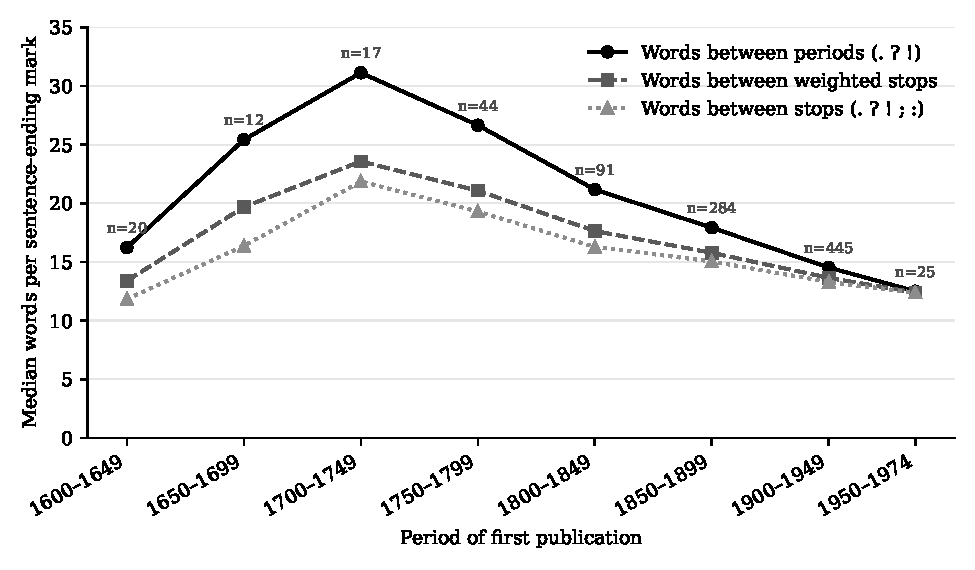
\includegraphics[width=0.85\linewidth,height=\textheight,keepaspectratio,alt={Median words between periods, between weighted stops and between all stops, by period of first publication, duplicates
removed. Weighted stops count each semicolon and colon at its glue rate (72\% and 59\%). Numbers above the points are books per period.}]{figure1.pdf}
\caption{Median words between periods, between weighted stops and between all stops, by period of first publication, duplicates removed. Weighted stops count each semicolon and colon at its glue rate
(72\% and 59\%). Numbers above the points are books per period.}
\end{figure}

Not every mark joins clauses. In the 82 English-original marks, 36 of 50 semicolons (72\%) and 19 of 32 colons (59\%) joined clauses that could stand alone. The others separated parallel
\emph{that}-clauses or relative clauses, introduced quotations or lists, or sat in headings and footnotes. On all 100 marks, the blind second coder agreed with the first on 95 (kappa 0.89); its rates
on the 82 English-original marks were 68\% and 56\%.

With duplicate works removed, P falls from 31.1 to 14.5 and the weighted S from 23.6 to 13.6. The punctuation share is 40\% (95\% interval 24--51\%). Almost all of the interval's width comes from the
17 books of 1700--1749: resampling books with the glue rates fixed gives 23--49\%. Under the second coder's rates (68\% and 56\%) the share is 39\% (22--49\%).

The 1900--1949 sample shows the marks partly changing jobs. Semicolons still mostly joined clauses (37 of 60, 62\%), but colons rarely did (7 of 40, 18\%): by then a colon mostly introduced a list or
a quotation. Weighting each era's books by its own sample's rates gives 41\% (25--53\%, resampling books and both samples' marks; \texttt{paper/era\_rates.py}), against 40\% with the 1700s rates
throughout. The 1900s rates rest on the single blind coder.

\subsection{Robustness}\label{robustness}

Table 3 gives the share under the variants that the per-book table supports, unweighted and weighted, with duplicates removed.

\needspace{15\baselineskip}

\begin{longtable}[]{@{}llrr@{}}
\caption{The punctuation share by variant, duplicates removed (\protect\texttt{paper/reanalysis.py}; the verified-originals rows from \protect\texttt{paper/verified\_originals.py}). Intervals resample
books (unweighted) or books and coded marks (weighted).}\tabularnewline
\toprule\noalign{}
Variant & Books (start/end) & Unweighted & Weighted \\
\midrule\noalign{}
\endfirsthead
\toprule\noalign{}
Variant & Books (start/end) & Unweighted & Weighted \\
\midrule\noalign{}
\endhead
\bottomrule\noalign{}
\endlastfoot
1700--1749 to 1900--1949 (main) & 17/445 & 48\% (33--61) & 40\% (24--51) \\
No plays or poetry & 16/426 & 52\% (36--60) & 41\% (26--50) \\
Translation flag removed & 12/395 & 59\% (51--64) & 47\% (37--53) \\
From 1750--1799 & 44/445 & 50\% (39--74) & 39\% (29--56) \\
All books, no deduplication & 18/445 & 47\% (39--60) & 38\% (29--50) \\
Verified English originals, 1700--1799 & 13/445 & 57\% (45--62) & 45\% (29--53) \\
Verified English originals, from 1750--1799 & 29/445 & 49\% (34--95) & 34\% (21--75) \\
\end{longtable}

The weighted variants in Table 3 range from 34\% to 47\%. Counting semicolons alone at their glue rate, with colons ignored, gives 37\% (18--47\%); this is a decomposition rather than a variant, since
colons that join clauses are part of the change. Weighting lowers each variant by 8 to 15 points, because the unweighted share counts marks that join nothing. The translation-flag variant is high, but
the flag both misses translations and removes English originals (Table 1). On the books verified as English originals the share is 45\% (29--53\%); among them the median P in 1700--1749 is 35.1 words
(13 books), against 31.1 for all 17. Starting at 1750 with verified originals gives 34\%, with an interval (21--75\%) too wide to read. The 1900--1949 books were not verified, but a translation from
that period is roughly contemporary with its original, so most of the distortion is at the early end. 45\% is therefore the better estimate for English-original prose; 40\% stays the main figure
because it requires no judgment about which books count.

The variants that need the full texts were rerun weighted and deduplicated (\texttt{paper/fulltext\_checks.py}). 55 of the 938 books have left Punc's shelf since the per-book table was made, so these
use the 883 that remain, on which the weighted base share is 42\% (26--51\%) rather than 40\%; Table 4 should be read against that base. Removing editorial apparatus changes little in the periods
compared: the median book with anything removed loses 0.1\% of its words in 1700--1749 and 0.2\% in 1900--1949. The largest change is in 1600--1649, outside the comparison, where P rises from 16.2 to
22.2.

\needspace{20\baselineskip}

\begin{longtable}[]{@{}llrr@{}}
\caption{Weighted punctuation share for the full-text variants, duplicates removed, 883 books (16 in 1700--1749, 43 in 1750--1799, 417 in 1900--1949). Intervals: 1,000 draws resampling books and coded
marks.}\tabularnewline
\toprule\noalign{}
Variant & Start & As is & Apparatus removed \\
\midrule\noalign{}
\endfirsthead
\toprule\noalign{}
Variant & Start & As is & Apparatus removed \\
\midrule\noalign{}
\endhead
\bottomrule\noalign{}
\endlastfoot
Base & 1700--1749 & 42\% (26--51) & 41\% (27--50) \\
Strict splitter & 1700--1749 & 43\% (28--53) & 43\% (29--53) \\
Dashes counted as stops & 1700--1749 & 39\% (20--50) & 39\% (22--51) \\
Narration only & 1700--1749 & 45\% (24--53) & 45\% (26--54) \\
Narration only, strict splitter & 1700--1749 & 49\% (26--57) & 48\% (28--57) \\
Narration only, single quotes removed too & 1700--1749 & 45\% (25--54) & 45\% (26--54) \\
Base & 1750--1799 & 39\% (26--59) & 35\% (26--58) \\
Strict splitter & 1750--1799 & 45\% (27--61) & 43\% (27--61) \\
Dashes counted as stops & 1750--1799 & 43\% (28--73) & 39\% (27--70) \\
Narration only & 1750--1799 & 39\% (19--66) & 36\% (16--67) \\
Narration only, strict splitter & 1750--1799 & 46\% (28--69) & 47\% (28--70) \\
Narration only, single quotes removed too & 1750--1799 & 40\% (23--69) & 41\% (20--71) \\
\end{longtable}

Every weighted full-text variant falls between 35\% and 49\%. The narration-only counts with the strict splitter are the highest, 6--7 points above the base from 1700 and up to 12 points above it from
1750. Unweighted, the same rows run from 48\% to 62\%.

\subsection{The remaining decline is not dialogue}\label{the-remaining-decline-is-not-dialogue}

The share of words inside quotation marks rises from 5\% in 1775--1799 to 26\% in 1800--1824 and then stays between 19\% and 34\% through 1974. Question marks rise from 1.9 to 5.3 per 1,000 words
between 1775--1799 and 1950--1974. With every quoted passage removed, median words between stops in narration still fall from 21.9 (1700--1749) to 14.5 (1900--1949), a fall of 7.4 words against 8.3
for the full text (both unweighted, before deduplication). On these figures, removing dialogue accounts for roughly a tenth of the decline in words between stops.

Weighted and deduplicated, the share on narration alone is 45\% (24--53\%), against 42\% for the full texts of the same 883 books (Table 4).

Two biases pull in opposite directions. Many eighteenth-century novels do not mark speech with quotation marks, which leaves short spoken lines in the early narration and understates narration's fall.
Many British books of 1900--1949 use single quotation marks, which leaves dialogue in the late narration and overstates its fall. The second is small: 21 of 417 books from 1900--1949 mostly use single
quotes, and removing single-quoted text as well moves narration's median P in that period from 16.5 to 16.6 and leaves the weighted narration share at 45\%. The single-quote rule also removes scare
quotes, which is why philosophy books such as \emph{Pragmatism} are among the 21. The first bias is not measured.

\subsection{The semicolon's decline}\label{the-semicolons-decline}

Sections 5.4 and 5.5 come from the original analysis: before deduplication, and with ``English original'' meaning the catalog's flag. Counting only 25-year periods with at least 20 books, the median
book has 10.1 semicolons per 1,000 words in 1775--1799, 12.6 in 1800--1824, 8.6 in 1850--1874, 4.6 in 1900--1924 and 1.8 in 1950--1974. Across 854 books dated from 1800, the least-squares slope is
−0.75 semicolons per 1,000 words per decade. As a share of all marks, the semicolon falls from 6.0\% to 0.8\% over the same periods. Commas fall less, from 85.9 to 63.1 per 1,000 words. The steepest
fall, after 1825, matches Rudnicka's (\citeproc{ref-Rudnicka2018}{2018}) American finding.

Darmon et al. (\citeproc{ref-Darmon2020}{2020}), also working with Project Gutenberg, describes the semicolon's fall as less pronounced in its full text. Measured as a share of all marks, the fall is
steep here too, so a per-word versus per-mark difference does not explain the gap. In that full text, Darmon et al. (\citeproc{ref-Darmon2020}{2020}) dates each work by its author's lifetime, since
Gutenberg does not record publication dates, and draws on a different slice of the library; these data cannot say which difference matters.

\subsection{Generations or publication dates}\label{generations-or-publication-dates}

If the semicolon's fall were a period effect, it should show up within careers, unless authors' own habits changed with age in the other direction. Among English originals with duplicates removed, 13
authors have five or more dated books spanning 20 or more years. Seven use fewer semicolons over their careers and six use more; the median slope is −0.06 per 1,000 words per decade (95\% interval
over authors −0.80 to +0.47). A pure period effect at the joint model's rate (below) would imply about −0.3 per decade. The interval includes both that and zero, so careers cannot decide between the
explanations.

Across 748 English-original books from 1750 to 1974, publication year alone and birth year alone fit about equally well (each −6.6 semicolons per 1,000 words per century; R² 0.273 and 0.275). In a
joint model the coefficients are −3.1 per century for publication year and −3.7 for birth year. With intervals from resampling 456 authors, they are −6.2 to −0.02 and −6.7 to −0.7. Holding birth year
fixed, publication year is also author age, so this is the age-period-cohort identification problem: the two predictors are nearly collinear and the model cannot apportion the decline between them. A
cohort effect of the kind Underwood et al. (\citeproc{ref-Underwood2022}{2022}) found for fiction is consistent with the data, and so is a period effect.

\section{Discussion}\label{discussion}

Between 1700--1749 and 1900--1949, the median stretch of prose between sentence-final marks fell by more than half, from 31.1 words to 14.5. Counting the semicolons and colons that join independent
clauses as boundaries, the median unit fell from 23.6 words to 13.6, a drop of about two fifths. In these Gutenberg texts, about 40\% of the decline between 1700--1749 and 1900--1949 is a change in
where writers, printers or later editors put periods. The rest is a real shortening of the units between stops, and it holds up when dialogue is removed. Neither unit splits independent clauses joined
by a comma and a conjunction, so the residual is not shown to be a shortening of clauses.

These results are consistent with Westin's (\citeproc{ref-Westin2002}{2002}) finding, as summarized in Rudnicka (\citeproc{ref-Rudnicka2018}{2018}), that the two ways of counting barely differ in
twentieth-century editorials: by then there are too few semicolons left to separate them. They also suggest that comparisons of sentence length across centuries should report a stop-based unit
alongside the orthographic sentence, or at least the semicolon rate.

Who moved the periods is a separate question. The career slopes, which cannot exclude either a period effect or none, and the equal fit of birth year and publication year allow both a generational
explanation (writers trained later used fewer semicolons) and a publishing one (houses and later editors repunctuated). Greg's (\citeproc{ref-Greg1950}{1950}) distinction between a text's substantive
readings and its accidentals is a reminder that punctuation is exactly what printers and editors felt free to change, which is the first limitation below.

\section{Limitations}\label{limitations}

\begin{itemize}
\tightlist
\item
  \textbf{Editions.} Gutenberg texts are often later editions, and editors change punctuation. Gutenberg's \emph{Wealth of Nations} reads ``hurtful to the landlord; it is frequently hurtful to the
  tenant; and it is always hurtful to the community,'' where the 1776 first edition has a period after ``landlord'' and a comma after ``tenant'' (\citeproc{ref-Smith1776}{Smith 1776}). That semicolon
  is item 5 of the coded sample. In this one documented case the later edition added a semicolon where the original had a period, which would raise early semicolon counts and inflate the punctuation
  share. Its size and direction across the corpus are unknown.
\item
  \textbf{Translations dated by the original.} A translation keeps the original's year but carries a translator's punctuation, often from a much later century. The catalog flag is unreliable in both
  directions (Table 1). The 1700--1799 books were checked against their title pages, and removing their translations raises the share to 45\%; books from 1800 on were not checked, so translations
  remain at the 1900--1949 end, and the generations model (Section 5.5) still relies on the catalog flag.
\item
  \textbf{Editorial apparatus.} Modern prefaces, editors' footnotes and glossaries are counted as period text in the main analysis, and the coded sample includes some (an editor's footnote in
  Franklin, a glossary in \emph{Gulliver's Travels}). Removing them by rule changes the share by one point from 1700 and four from 1750 (Table 4), but rules miss notes set inline without markers.
\item
  \textbf{Model coding.} Both coders are runs of one model family; the first knew the hypothesis and the result; the 1900s sample has a single coder. A human coder, ideally a historical linguist,
  coding both samples blind is the most important check this paper lacks. A blind coding page and a scorer for that are published in \texttt{paper/coding/}.
\item
  \textbf{One glue rate for all books.} Each mark's rate comes from a pooled sample of 82 marks; it does not vary by book, author or genre, or by period except in the one check with the 1900s sample's
  rates.
\item
  \textbf{Small early periods.} After deduplication, the 50-year periods before 1800 have 12 to 44 books, and the intervals are wide.
\item
  \textbf{Start period.} 1700--1749 is the peak of P for the whole shelf but not for prose alone, where the 10 books from 1600--1649 run longer.
\item
  \textbf{No recent books.} Only 67 dated books appeared after 1930.
\item
  \textbf{The live shelf drifts.} 55 of the 938 books have left Punc's shelf since the snapshot; on the 883 that remain the base share is 42\%, not 40\%. The published book list fixes the corpus.
\item
  \textbf{Half the shelf is undated.} 1,073 of 1,959 books have a first-publication year; whether undated books differ is untested.
\item
  \textbf{Today's taste.} The shelf is chosen by current download counts (Section 3).
\item
  \textbf{Dialogue.} Narration-only counts remove double- and single-quoted text; speech that eighteenth-century novels leave unmarked, and the speech in plays, stays in (Section 5.3).
\item
  \textbf{Correlation only.} Nothing here establishes why writers or printers changed.
\end{itemize}

\section{Data and code availability}\label{data-and-code-availability}

Punc's counting code (TypeScript) and site are at \url{https://github.com/JoeKarlsson/punc}. The Python analysis scripts (standard library only), the per-book table (\texttt{analysis/books.csv}), both
coded samples, the second coder's prompt and a ledger of every number from the original analysis (\texttt{analysis/RESULTS.md}) are in the repository's \texttt{analysis/} folder. The deduplication,
the recomputed glue rates and Table 3 come from \texttt{paper/reanalysis.py} (its output is \texttt{paper/reanalysis-output.md}), and Table 1 from \texttt{paper/corpus\_table.py}. The verified
translation status and its shares are in \texttt{paper/translation-status.csv} and \texttt{paper/verified\_originals.py}; Table 4 and the single-quote counts come from
\texttt{paper/fulltext\_checks.py}; Figure 1 from \texttt{paper/figure1.py}; the era-specific rates from \texttt{paper/era\_rates.py}. The analysis reads the frozen per-book table
\texttt{analysis/books.csv}, built from the 1,959-book shelf of 2026-11-10 (the last commit with that shelf is 5a2b926), and Gutenberg's catalog downloaded the same day. A Zenodo deposit with a DOI
will accompany submission.

\section*{References}\label{references}
\addcontentsline{toc}{section}{References}

\protect\phantomsection\label{refs}
\begin{CSLReferences}{1}{1}
\bibitem[\citeproctext]{ref-Biber2009}
Biber, Douglas, and Susan Conrad. 2009. \emph{Register, Genre, and Style}. Cambridge University Press. \url{https://doi.org/10.1017/cbo9780511814358}.

\bibitem[\citeproctext]{ref-Biber1989}
Biber, Douglas, and Edward Finegan. 1989. {``Drift and the Evolution of English Style: A History of Three Genres.''} \emph{Language} 65 (3): 487--517. \url{https://doi.org/10.2307/415220}.

\bibitem[\citeproctext]{ref-Biber2015}
Biber, Douglas, and Bethany Gray. 2015. \emph{Grammatical Complexity in Academic English: Linguistic Change in Writing}. Cambridge University Press. \url{https://doi.org/10.1017/cbo9780511920776}.

\bibitem[\citeproctext]{ref-Bruthiaux1995}
Bruthiaux, P. 1995. {``The Rise and Fall of the Semicolon: English Punctuation Theory and English Teaching Practice.''} \emph{Applied Linguistics} 16 (1): 1--14.
\url{https://doi.org/10.1093/applin/16.1.1}.

\bibitem[\citeproctext]{ref-Cohen1960}
Cohen, Jacob. 1960. {``A Coefficient of Agreement for Nominal Scales.''} \emph{Educational and Psychological Measurement} 20 (1): 37--46. \url{https://doi.org/10.1177/001316446002000104}.

\bibitem[\citeproctext]{ref-Darmon2020}
Darmon, Alexandra N. M., Marya Bazzi, Sam D. Howison, and Mason A. Porter. 2020. {``Pull out All the Stops: Textual Analysis via Punctuation Sequences.''} \emph{European Journal of Applied
Mathematics} 32 (6): 1069--105. \url{https://doi.org/10.1017/s0956792520000157}.

\bibitem[\citeproctext]{ref-Domain2026}
Duke Center for the Study of the Public Domain. 2026. {``Public Domain Day 2026.''} \url{https://cspd.law.duke.edu/publicdomainday/2026}.

\bibitem[\citeproctext]{ref-Efron1979}
Efron, B. 1979. {``Bootstrap Methods: Another Look at the Jackknife.''} \emph{The Annals of Statistics} 7 (1): 1--26. \url{https://doi.org/10.1214/aos/1176344552}.

\bibitem[\citeproctext]{ref-Fahnestock2011}
Fahnestock, Jeanne. 2011. \emph{Rhetorical Style: The Uses of Language in Persuasion}. Oxford University Press. \url{https://doi.org/10.1093/acprof:oso/9780199764129.001.0001}.

\bibitem[\citeproctext]{ref-Gerlach2020}
Gerlach, Martin, and Francesc Font-Clos. 2020. {``A Standardized Project Gutenberg Corpus for Statistical Analysis of Natural Language and Quantitative Linguistics.''} \emph{Entropy} 22 (1): 126.
\url{https://doi.org/10.3390/e22010126}.

\bibitem[\citeproctext]{ref-Gilardi2023}
Gilardi, Fabrizio, Meysam Alizadeh, and Maël Kubli. 2023. {``ChatGPT Outperforms Crowd Workers for Text-Annotation Tasks.''} \emph{Proceedings of the National Academy of Sciences} 120 (30).
\url{https://doi.org/10.1073/pnas.2305016120}.

\bibitem[\citeproctext]{ref-Greg1950}
Greg, W. W. 1950. {``The Rationale of Copy-Text.''} \emph{Studies in Bibliography} 3: 19--36.

\bibitem[\citeproctext]{ref-Hunt1965}
Hunt, Kellogg W. 1965. \emph{Grammatical Structures Written at Three Grade Levels}. NCTE Research Report 3. National Council of Teachers of English.

\bibitem[\citeproctext]{ref-Kulig2016}
Kulig, Andrzej, Jarosław Kwapień, Tomasz Stanisz, and Stanisław Drożdż. 2017. {``In Narrative Texts Punctuation Marks Obey the Same Statistics as Words.''} \emph{Information Sciences} 375 (January):
98--113. \url{https://doi.org/10.1016/j.ins.2016.09.051}.

\bibitem[\citeproctext]{ref-Lewis1894}
Lewis, Edwin Herbert. 1894. \emph{The History of the English Paragraph}. University of Chicago Press. \url{https://archive.org/details/historyenglishp00lewigoog}.

\bibitem[\citeproctext]{ref-Liberman2022}
Liberman, Mark. 2022. {``Historical Trends in English Sentence Length and Syntactic Complexity.''} \url{https://languagelog.ldc.upenn.edu/myl/LibermanSHEL12.pdf}.

\bibitem[\citeproctext]{ref-Muzny2017}
Muzny, Grace, Mark Algee-Hewitt, and Dan Jurafsky. 2017. {``Dialogism in the Novel: A Computational Model of the Dialogic Nature of Narration and Quotations.''} \emph{Digital Scholarship in the
Humanities} 32 (suppl\_2): ii31--52. \url{https://doi.org/10.1093/llc/fqx031}.

\bibitem[\citeproctext]{ref-Nunberg1990}
Nunberg, Geoffrey. 1990. \emph{The Linguistics of Punctuation}. CSLI Lecture Notes 18. {Center for the Study of Language and Information}.

\bibitem[\citeproctext]{ref-Oliver2025}
Oliver, Henry. 2025. {``The Triumph of Logical English.''} Works in Progress. \url{https://worksinprogress.co/issue/the-logical-triumph-of-english/}.

\bibitem[\citeproctext]{ref-Parkes1992}
Parkes, M. B. 1992. \emph{Pause and Effect: An Introduction to the History of Punctuation in the West}. Scolar Press.

\bibitem[\citeproctext]{ref-Rudnicka2018}
Rudnicka, Karolina. 2018. {``Variation of Sentence Length across Time and Genre: Influence on Syntactic Usage in English.''} In \emph{Diachronic Corpora, Genre, and Language Change}. John Benjamins
Publishing Company. \url{https://doi.org/10.1075/scl.85.10rud}.

\bibitem[\citeproctext]{ref-Ryder1965}
Ryder, Norman B. 1965. {``The Cohort as a Concept in the Study of Social Change.''} \emph{American Sociological Review} 30 (6): 843--61. \url{https://doi.org/10.2307/2090964}.

\bibitem[\citeproctext]{ref-Sherman1893}
Sherman, L. A. 1893. \emph{Analytics of Literature: A Manual for the Objective Study of English Prose and Poetry}. Ginn \& Company. \url{https://archive.org/details/analyticsofliter00sheruoft}.

\bibitem[\citeproctext]{ref-Smith1776}
Smith, Adam. 1776. \emph{An Inquiry into the Nature and Causes of the Wealth of Nations}. {W. Strahan and T. Cadell}. \url{https://archive.org/details/inquiryintonatur02smit_0}.

\bibitem[\citeproctext]{ref-Stanisz2023}
Stanisz, Tomasz, Stanisław Drożdż, and Jarosław Kwapień. 2023. {``Universal versus System-Specific Features of Punctuation Usage Patterns in Major Western Languages.''} \emph{Chaos, Solitons \&
Fractals} 168 (March): 113183. \url{https://doi.org/10.1016/j.chaos.2023.113183}.

\bibitem[\citeproctext]{ref-Tornberg2023}
Törnberg, Petter. 2023. {``{ChatGPT-4} Outperforms Experts and Crowd Workers in Annotating Political {Twitter} Messages with Zero-Shot Learning.''} arXiv.
\url{https://doi.org/10.48550/arXiv.2304.06588}.

\bibitem[\citeproctext]{ref-Underwood2022}
Underwood, Ted, Kevin Kiley, Wenyi Shang, and Stephen Vaisey. 2022. {``Cohort Succession Explains Most Change in Literary Culture.''} \emph{Sociological Science} 9: 184--205.
\url{https://doi.org/10.15195/v9.a8}.

\bibitem[\citeproctext]{ref-Vrandecic2014}
Vrandečić, Denny, and Markus Krötzsch. 2014. {``Wikidata: A Free Collaborative Knowledgebase.''} \emph{Communications of the ACM} 57 (10): 78--85. \url{https://doi.org/10.1145/2629489}.

\bibitem[\citeproctext]{ref-Watson2019}
Watson, Cecelia. 2019. \emph{Semicolon: The Past, Present, and Future of a Misunderstood Mark}. Ecco.

\bibitem[\citeproctext]{ref-Westin2002}
Westin, Ingrid. 2002. \emph{Language Change in English Newspaper Editorials}. BRILL. \url{https://doi.org/10.1163/9789004334007}.

\end{CSLReferences}

\end{document}
